% !TeX root = ../main.tex
\chapter{用户输入意图推理算法探究}
\label{cha:algorithm}
\section{方法设计}
在本章中,我们通过上个实验收集的用户在桌面上的点击数据,进行模拟实验,试图探究能够预测用户输入单词的推理算法。

对于每一种算法,我们的输入为用户的点击位置信息,输出为该算法预测出的概率最高的五个可能的单词。然后将其与正确的单词进行比对,分别计算对应的概率第一高到概率第五高的单词级别准确率。我们使用的是美国国家语料库,其中收录了各种正式和非正式场景下超过了2,000万个单词。从该语料库中我们挑选了出现频率最高的10,000个单词作为词库,作为计算单词出现的概率。我们保证用户在上个实验中输入的单词都出现在词库中。

\section{算法选择}
在文献综述部分,我们提到虚拟键盘上通常使用的纠错算法都是基于贝叶斯原理,包括绝对位置和相对位置两种。相对位置的纠错算法也有两种形式,一是当一只手或者一个手指负责整个键盘时,研究者直接计算两次点击的位置变化;二是当用户使用两只手输入时,通常将两手的位置变化分开考虑,即计算一个单词的出现概率时,将一连串点击归类为左右手分别计算,最后相乘。然而,用户在十指盲打时,尤其是在我们的场景中是双手抬起,两只手的运动是一个整体,并不相互独立,因此点击也有可能呈现第一种相对位置运动规律,即仍然直接计算连续点击的位置变化。从而我们一共有三种推理算法,分别称为绝对模型、全键盘相对模型、半键盘相对模型。使用公式~(\ref{equ:fitkeyboard})~对三种点击模型进行拟合,表~\ref{tab:modelr2}~的结果显示所有的点击模型拟合$R^2$都超过了0.80,并且相对模型下对于纵轴的拟合效果更好,说明用户在纵轴的点击规律更符合相对模型。

\begin{table}[htb]
  \centering
  \begin{minipage}[t]{0.6\linewidth} % 如果想在表格中使用脚注,minipage是个不错的办法
  \caption[三种点击模型拟合的$R^{2}$]{三种点击模型拟合的$R^{2}$}
  \label{tab:modelr2}
    \centering
    \begin{tabularx}{\linewidth}{cccc}
      \toprule[1.5pt]
      %  & \multicolumn{2}{c}{总体}&\multicolumn{2}{c}{左手} &  \multicolumn{2}{c}{右手} \\\midrule[1pt]
      & 绝对模型 & 全键盘相对模型 & 半键盘相对模型 \\\midrule[1pt]
      X & 0.96 (0.01) & 0.95 (0.01) & 0.82 (0.02) \\
      Y & 0.85 (0.01) & 0.89 (0.01) & 0.91 (0.02)\\
      \bottomrule[1.5pt]
    \end{tabularx}
  \end{minipage}
\end{table}

此外,对于每一种点击模型,我们计算了单人和整体两种情况下的准确率。其中单人指的是将每个人的落点分别计算准确率后平均,整体指的是将所有人的落点合并并且平移后计算总准确率。在实际使用中,因为一开始缺乏用户个性化的数据,所以总是从整体出发。

\section{模拟结果}
不同情况下的准确率如图~\ref{fig:simulation}。可以看到,所有情况下的概率第一高的准确率都超过了80\%。对于不同的模型,单人平均值总是好于总体,因为每个人的点击规律并不相同,将按键平移后会增加不准确性,从而降低预测准确率。

\begin{figure}[h] % use float package if you want it here
    \centering
    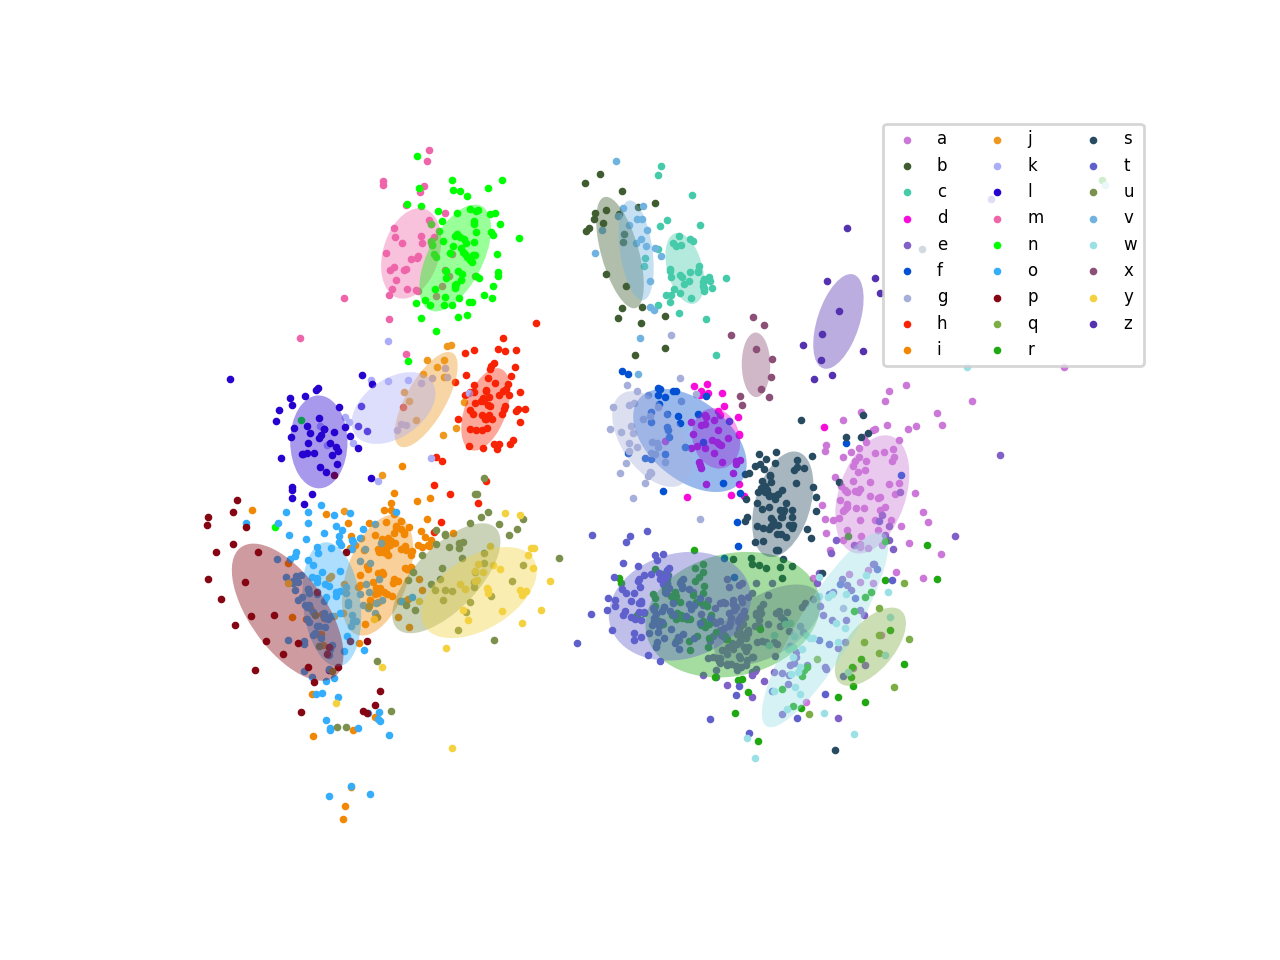
\includegraphics[width=8cm]{touchpoints.png}
    \caption{不同算法模拟的准确率}
    \label{fig:simulation}
\end{figure}